% \documentclass[12pt]{article}
\documentclass[12pt]{ctexart}
\usepackage[utf8]{inputenc}

\usepackage[english]{babel}
\usepackage[dvips]{epsfig}
\usepackage{amsmath}
\usepackage{amssymb}
\usepackage{amsfonts}
\usepackage{amsthm}
\usepackage{amsbsy}
\usepackage{amsgen}
\usepackage{amscd}
\usepackage{amsopn}
\usepackage{amstext}
\usepackage{amsxtra}
\usepackage{mathrsfs}
\usepackage{enumitem}
\usepackage{graphicx}
\usepackage{verbatim}
\usepackage{epstopdf}
\usepackage{float}
\usepackage[all,cmtip]{xy}
\usepackage{accents}
\usepackage{sseq}
\usepackage{url}
\usepackage{hyperref}
\usepackage{makeidx}
\usepackage{siunitx}
\usepackage{xcolor}
\usepackage{physics}

%%%%%%%%% 版面设置 %%%%%%%%%%%%%%%%%%%%%%%%%%%%%%%%%%%%%%
\usepackage{geometry}
\usepackage{titlesec}
\usepackage{fancyhdr}\pagestyle{empty}
\titleformat*{\section}{\large\bfseries}

%
\geometry{
	a4paper,
	total={170mm,240mm},
	left=20mm,
	top=30mm,
}

%Bitte nicht einstellen
\renewcommand{\figurename}{Abbildung}
\renewcommand{\tablename}{Tabelle}
\pagestyle{fancyplain}
\headheight 35pt
\lhead{\name}
\chead{\textbf{\Large \Title}}
\rhead{\due\\\today}
\lfoot{}
\cfoot{}
\rfoot{\small\thepage}
\headsep 1.5em

%%%%%%%%%%%%%%%%%%%%%%%%%%%%%%%%%%%%%%%%%%%%%%%%%%%%%%

\newtheorem{thm}{Theorem}[section]

% 定义解题环境
\theoremstyle{remark}
\newtheorem{remark}[thm]{Remark}
\newtheorem{theorem}{Theorem}
\newtheorem{observation}[thm]{Observation}

\theoremstyle{definition}
\newtheorem{problem}{\text{}}
\newtheorem{Problem}{\text{Problem}}
\newtheorem*{solution}{解}
\newtheorem*{Answer}{Answer}
\newtheorem{example}{Example} 

%%%%%%%%%%%%%%%%%%%%%%%%%%%%%%%%%%%%%%%%%%%%%%%%%%%%%%%%%%%%%%%%%%
\newcommand\name{陈景龙22120307}
\newcommand\due{-}
\newcommand{\emptyline}{\vspace{0.6\baselineskip}}

\usepackage{tikz}

\newcommand{\Title}{CVX HW}
\renewcommand{\due}{due: 11 weeks}
\newcommand{\tr}{\operatorname{tr}} % 迹
\newcommand{\dom}{\operatorname{dom}} % 定义域
\newcommand{\minimize}{\operatorname{minimize}} % 最小化
\newcommand{\subject}{\operatorname{subject\ to}}

\newcommand{\todo}{{\color{red} to do}} % to do
\newcommand{\myline}{{\line(1,0){450}}} % 分割线

% 自定义 enumerate
\renewcommand{\labelenumi}{(\alph{enumi})}

\begin{document}
\section{Convex sets}
\begin{problem}[2.1]
    Let $C \subseteq \mathbb{R}^{n}$ be a convex set, with $x_1, \dots, x_k \in C$, and let $\theta_1, \dots, \theta_k \in \mathbb{R}$ satisfy $\theta_i \ge 0$, $\theta_1 + \cdots + \theta_k = 1$. Show that $\theta_1x_1 + \cdots + \theta_kx_k \in C$.(The definition of convexity is that this holds for $k = 2$; you must show it for arbitrary k.) \textit{Hint.} Use induction on k.

    \begin{proof}
        \text{}
        \begin{itemize}
            \item When $k = 2$, $\theta_i \ge 0, \theta_1 + \theta_2 = 1 \Longrightarrow \theta_1 x_1 + \theta_2x_2 = \theta_1 x_1 + (1 - \theta_1)x_2 \in C$.
            \item If $k = n$, $\theta_i \ge 0, \theta_1 + \cdots + \theta_n = 1 \Longrightarrow \theta_1x_1 + \cdots + \theta_nx_n \in C$ holds.
            \item Then $k = n + 1$, $\theta_i \ge 0, \theta_1 + \cdots + \theta_{n + 1} = 1 \Longrightarrow \theta_1x_1 + \cdots + \theta_nx_n + \theta_{n + 1}x_{n + 1} = (\theta_1 + \cdots + \theta_n)\frac{\theta_1x_1 + \cdots + \theta_nx_n}{\theta_1 + \cdots + \theta_n} + \theta_{n + 1}x_{n + 1}$. $k = n, \theta_1x_1 + \cdots + \theta_nx_n \in C$ holds, and $k = 2$ holds, so $\theta_1x_1 + \cdots + \theta_nx_n + \theta_{n + 1}x_{n + 1} \in C$.
            \item so $\theta_1x_1 + \cdots + \theta_kx_k \in C$ for arbitrary $k$.
        \end{itemize}
    \end{proof}
\end{problem}

\begin{problem}[2.5]
    What is the distance between two parallel hyperplanes $\left\{x \in \mathbb{R}^n | a^Tx = b_1\right\}$ and $\left\{x \in \mathbb{R}^n| \right.$ $\left. a^Tx = b_2\right\}$?

    \Answer The distance between the two hyperplanes is $\frac{|b_1 - b_2|}{\|a\|_2}$.
\end{problem}

\begin{problem}[2.11]
    \textit{Hyperbolic sets.} Show that the \textit{Hyperbolic set} $\left\{x \in \mathbb{R}_+^2 | x_1x_2 \ge 1\right\}$ is convex. As a generalization, show that $\left\{x \in \mathbb{R}^n_+ | \prod_{i = 1}^n x_i \ge 1\right\}$ is convex. \textit{Hint.} If $a, b \ge 0$ and $0 \le \theta \le 1$, then $a^\theta b^{1 - \theta} \le \theta a + (1 - \theta)b$.
    
    \Answer \begin{enumerate}
        \item $x, y \in C$, then $z = \theta x + (1 - \theta)y$.
        \begin{align*}
            z_1z_2 &= (\theta x_1 + (1 - \theta)y_1)(\theta x_2 + (1 - \theta)y_2) \\
            &\ge x_1^\theta y_1^{1 - \theta} \cdot x_2^\theta y_2^{1 - \theta} \\
            &= (x_1x_2)^\theta (y_1y_2)^{1 - \theta}\\
            &\ge 1
        \end{align*}
        we get $z \in C$ and $\left\{x \in \mathbb{R}_+^2 | x_1x_2 \ge 1\right\}$ is convex.
        \item $x, y \in C$, then $z = \theta x + (1 - \theta)y$.
        \begin{align*}
            z_1z_2 &= \prod_{i = 1}^n(\theta x_i + (1 - \theta)y_i)\\
            &\ge \prod_{i = 1}^n x_i^\theta y_i^{1 - \theta} \\
            &\ge 1
        \end{align*}
        we get $z \in C$ and $\left\{x \in \mathbb{R}^n_+ | \prod_{i = 1}^n x_i \ge 1\right\}$ is convex.
    \end{enumerate}
\end{problem}

\begin{problem}[2.14]
    \textit{Erpanded and restricted sets.} Let $S \subseteq \mathbb{R}^{n}$, and let $\|\cdot\|$ be a norm on $\mathbb{R}^n$.
    \begin{enumerate}
        \item For $a \ge 0$ we define $S_a$ as $\{x \mid \operatorname{dist}(x, S) \leq a\}$, where $\operatorname{dist}(x, S) = \inf_{y\in S}\|x - y\|$. We refer to $S_a$ as $S$ \textit{expanded} or \textit{extended} by $a$. Show that if $S$ is convex, then $S_a$ is convex.
        \item For $a \ge 0$ we define $S_{-a} = \left\{x | B(x, a) \subseteq S\right\}$, where $B(x, a)$ is the ball (in the norm $\|\cdot\|$), centered at x, with radius a. We refer to $S_{-a}$ as $S$ \textit{shrunk} or \textit{restricted} by $a$, since $S_{-a}$ consists of all points that are at least a distance a from $\mathbb{R}^n\backslash S$. Show that if $S$ is convex, then $S_{-a}$ is convex.
    \end{enumerate}

    \begin{proof}
        \begin{enumerate}
            \item $\forall x_1, x_2 \in S_a$, for $0 \le \theta \le 1$, $z = \theta x_1 + (1 - \theta)x_2$
            \begin{align*}
                \operatorname{dist}(z, S) &= \inf_{y\in S}\|z - y\|\\
                &= \inf_{y_1, y_2\in S}\|\theta x_1 + (1 - \theta)x_2 - \theta y_1 - (1 - \theta)y_2\|\\
                &\le \inf_{y_1, y_2\in S} (\theta\|x_1 - y_1\| + (1 - \theta)\|x_2 - y_2\|)\\
                &=\theta \inf_{y_1 \in S}\|x_1 - y_1\| + (1 - \theta) \inf_{y_2 \in S} \|x_2 - y_2\|\\
                &\le a
            \end{align*}
            so $\forall x_1, x_2 \in S_a, z \in S_a$, $S_{a}$ is convex.
            \item Consider $x_1, x_2 \in S_{-a}$, $\forall u$ with $\|u\| \le a$,\[x_1 + u \in S,\quad x_2 + u \in S\] $\forall \theta \in [0, 1], \|u\| \le a$,
            \[z + u = \theta x_1 + (1 - \theta)x_2 + u = \theta(x_1 + u) + (1 - \theta)(x_2 + u) \in S\]
            because $S$ is convex. We conclude that $z \in S_{-a}$.
        \end{enumerate}
    \end{proof}
\end{problem}

\section{Convex functions}
\begin{problem}[3.1]
    Suppose $f: \mathbb{R} \to \mathbb{R}$ is convex, and $a, b \in \dom(f)$ with $a < b$.
    \begin{enumerate}
        \item Show that \[f(x) \le \frac{b - x}{b - a}f(a) + \frac{x - a}{b - a}f(b)\] for all $x \in [a, b]$.
        \item Show that \[\frac{f(x) - f(a)}{x - a} \le \frac{f(b) - f(a)}{b - a} \le \frac{f(b) - f(x)}{b - x}\] for all $x \in (a, b)$. Draw a sketch that illustrates this inequality. 
        \item Suppose f is differentiable. Use the result in (b) to show that \[f^\prime(a) \le \frac{f(b) - f(a)}{b - a} \le f^\prime(b)\] Note that these inequalities also follow from:\[f(b) \ge f(a) + f^\prime(a)(b - a) \]
        \item Suppose $f$ is twice differentiable. Use the result in (c) to show that $f^{\prime \prime}(a) \geq 0$ and $f^{\prime \prime}(b) \geq 0$.
    \end{enumerate}

    \begin{proof}
        \text{}
        \begin{enumerate}
            \item $f$ is convex, so $f(\theta x_1 + (1 - \theta)x_2) \le \theta f(x_1) + (1 - \theta)f(x_2)$. When $x = \theta x_1 + (1 - \theta)x_2$, $a = x_1, b = x_2$, we get $\theta = \frac{x_2 - x}{x_2 - x_1}$, so \[f(x) \le \frac{b - x}{b - a}f(a) + \frac{x - a}{b - a}f(b)\] for all $x \in [a, b]$
            \item \begin{align*}
                f(x) &\le \frac{b - x}{b - a}f(a) + \frac{x - a}{b - a}f(b) \\
                f(x) - f(a) &\le \frac{b - x}{b - a}f(a) + \frac{x - a}{b - a}f(b) - f(a) \\
                \frac{f(x) - f(a)}{x - a} &\le \frac{f(b) - f(a)}{b - a}
            \end{align*}
            So the left inequality holds. The inequality on the right is the same.
            \[\frac{f(x) - f(a)}{x - a} \le \frac{f(b) - f(a)}{b - a} \le \frac{f(b) - f(x)}{b - x}\]
            Geometrically, in figure \ref{fig1} the inequalities mean that $k_{ax} < k_{ab} < k_{xb}$, $k_{ab}$ means the slope of the line segment between $(a, f(a))$ and $(b, f(b))$.
            \begin{figure}[htbp]
                \centering
                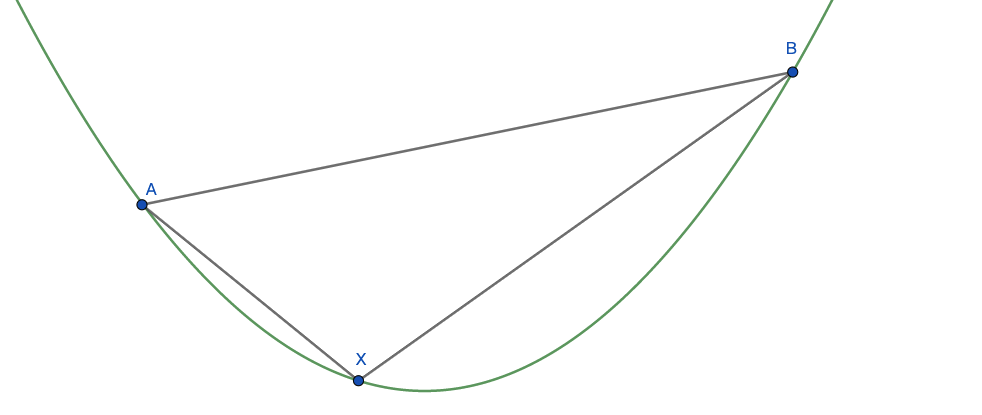
\includegraphics[width=0.6\textwidth]{./figure/fig1.png}
                \caption{sketch that illustrates this inequality \label{fig1}}
            \end{figure}
        \end{enumerate}
    \end{proof}
\end{problem}

\begin{problem}[3.7]
    Suppose $f : \mathbb{R}^n \to \mathbb{R}$ is convex with $\dom(f) = \mathbb{R}^n$. and bounded above on $\mathbb{R}^n$. Show that f is constant.

    \Answer Suppose $f$ is not constant. $\exists x, y$, s.t. $f(x) < f(y)$.
    \[g(t) = f(tx + (1 - t)y)\] is convex, $g(0) = f(y) > f(x) = g(1)$. We get
    \[g(0) \le \frac{t - 1}{t}g(1) + \frac{1}{t}g(t)\] for all $t > 1$, and
    \[g(t) \ge tg(0) - (t - 1)g(1) = g(1) + t(g(0) - g(1))\]
    so $g$ grows unboundedly as $t \to \infty$. This contradicts our assumption that $f$ is bounded. So $f$ is constant.
\end{problem}

\begin{problem}[3.16]
    For each of the following functions determine whether it is convex, concave, quasiconvex, or quasiconcave.(consider only convexity and concavity)
    \begin{enumerate}
        \item $f(x) = e^x - 1$ on $\mathbb{R}$.
        \item $f(x_1, x_2) = x_1x_2$ on $\mathbb{R}^2_{++}$.
        \item $f(x_1, x_2) = 1 / (x_1x_2)$ on $\mathbb{R}^2_{++}$.
        \item $f(x_1, x_2) = x_1/x_2$ on $\mathbb{R}^2_{++}$.
        \item $f(x_1, x_2) = x_1^2/x_2$ on $\mathbb{R}\times \mathbb{R}_{++}$.
        \item $f(x_1, x_2) = x_1^\alpha x_2^{1 - \alpha}$, where $0\le \alpha \le 1$, on $\mathbb{R}^2_{++}$.
    \end{enumerate}

    \Answer \text{}\begin{enumerate}
        \item $f^{\prime\prime}(x) = e^x > 0$, so $f$ is convex but not concave.
        \item $\nabla^2 f = \begin{pmatrix}
            0 & 1 \\
            1 & 0
        \end{pmatrix}$ is neither positive semidefinite nor negative semidefinite, so $f$ is neither convex nor concave.
        \item $\nabla^2f = \frac{1}{x_1^3x_2^3}\begin{pmatrix}
            2x_2^2 & x_1x_2 \\
            x_1x_2 & 2x_1^2
        \end{pmatrix} \succeq 0$, so $f$ is convex but not concave.
        \item $\nabla^2f = \frac{1}{x_2^3}\begin{pmatrix}
            0 & -x_2\\
            -x_2 & 2x_1
        \end{pmatrix}$ is neither positive semidefinite nor negative semidefinite, so $f$ is neither convex nor concave.
        \item $\nabla^2f = \frac{2}{x_2^3}\begin{pmatrix}
            x_2^2 & -x_1x_2 \\
            -x_1x_2 & x_1^2
        \end{pmatrix} \succeq 0$, so $f$ is convex but not concave.
        \item \begin{align*}    
            \nabla^2f &= \alpha(1 - \alpha)\begin{pmatrix}
                x_1^{\alpha - 2}x_2^{1 - \alpha} & -x_1^{\alpha - 1}x_2^{-\alpha}\\
                -x_1^{\alpha - 1}x_2^{-\alpha} & -x_1^\alpha x_2^{-\alpha - 1}
            \end{pmatrix}\\ 
            &=\alpha(1 - \alpha)x_1^{\alpha}x_2^{1 - \alpha}\begin{pmatrix}
                -1 / x_1^2 & 1 / x_1x_2 \\
                1 \ x_1x_2 & -1 / x_2^2
            \end{pmatrix}\\
            &=-\alpha(1 - \alpha)x_1^{\alpha}x_2^{1 - \alpha}\begin{pmatrix}
                1 / x_1 \\
                -1 / x_2
            \end{pmatrix}\begin{pmatrix}
                1 / x_1 & -1 / x_2
            \end{pmatrix}\\
            &\preceq 0
        \end{align*}
        so $f$ is concave but not convex.
    \end{enumerate}
\end{problem}

\begin{problem}[3.18]
    Adapt the proof of concavity of the log-determinant function in $\S 3.1.5$ to show the following.
    \begin{enumerate}
        \item $f(X) = \tr(X^{-1})$ is convex on $\dom(f) = \mathbb{R}^n_{++}$.
        \item $f(X) = (\operatorname{det} X)^{1 / n}$ is concave on $\dom(f) = \mathbb{R}^n_{++}$.
    \end{enumerate}

    \Answer \text{}
    \begin{enumerate}
        \item Define $g(t) = f(Z + tV)$, where $Z \succ 0$ and $V \in \mathbb{S}^n$. \begin{align*}
            g(t) &= \tr((Z + tV)^{-1})\\
            &= \tr(Z^{-1}(I + tZ^{-\frac{1}{2}}VZ^{-\frac{1}{2}})^{-1})\\
            &= \tr(Z^{-1} Q (I + t\Lambda)^{-1} Q^t)\\
            &= \tr(Q^tZ^{-1}Q(I + t\Lambda)^{-1})\\
            &= \sum_{i = 1}^n(Q^tZ^{-1}Q)_{ii}(1 + t\lambda_i)^{-1}
        \end{align*}
        We express $g$ as a positive weighted sum of convex functions $\frac{1}{1 + t\lambda_i}$, hence it is convex.
        \item Define $g(t) = f(Z + tV)$, where $Z \succ 0$ and $V \in \mathbb{S}^n$. \begin{align*}
            g(t) &= (\det(Z + tV))^{\frac{1}{n}}\\
            &= (\det(Z^{\frac{1}{2}}) \det(I + tZ^{-\frac{1}{2}}VZ^{-\frac{1}{2}}) \det(Z^{\frac{1}{2}}))^{\frac{1}{2}}\\ 
            &= (\det(Z))^{\frac{1}{n}}\left(\prod_{i = 1}^n(1 + t\lambda_i)\right)^{\frac{1}{n}}
        \end{align*}

        where $\lambda_i$ are the eigenvalues of $Z^{-\frac{1}{2}} V Z^{-\frac{1}{2}}$. We see that $g$ is a concave function of $t$ on $\left\{t \ | \ Z + tV \succ 0\right\}$, since $\det(Z) > 0$ and the geometric mean $(\prod_{i = 1}^nx_i)^{\frac{1}{n}}$ is concave on $\mathbb{R}_{++}^n$.
    \end{enumerate}
\end{problem}


\begin{problem}[3.27]
    \textit{Diagonal elements of Cholesky factor.} Each $X \in \mathbf{S}^n_{++}$ has a unique \textit{Cholesky factorization} $X = LL^T$, where $L$ is lower triangular, with $L_{ii} > 0$. Show that $L_{ii}$ is a concave function of $X$ (with domain $\mathbf{S}^n_{++}$).

    \textit{Hint.} $L_{ii}$ can be expressed as $L_{ii} = (w - z^tY^{-1}z)^{1 / 2}$, where\[\begin{bmatrix}
        Y & z \\
        z^T & w
    \end{bmatrix}\] is the leading $i \times i$ submatrix of $X$.

    \Answer $f(z, Y) = z^tY^{-1}z$ with $\dom(f) = \left\{(z, Y) | Y \succ 0\right\}$ is convex jointly in $z$ and $Y$. Notice that \[(z, Y, t) \in \operatorname{epi}(f) \quad \Longleftrightarrow \quad Y \succ 0, \quad\begin{bmatrix}
        Y & z \\
        z^t & T
    \end{bmatrix} \succeq 0\] so $\operatorname{epi}(f)$ is a convex set. Therefore, $w - z^tY^{-1}z$ is a concave function of $X$. Since the squareroot is an increasing concave function, it follows from the composition rules that $l_{kk} = (w - z^tY^{-1}z)^{\frac{1}{2}}$ is a concave function of $X$.
\end{problem}


\begin{problem}[3.31]
    \textit{Largest homogeneous und restimator.}Let $f$ be a convex function. Define the function $g$ as 
    \[g(x)=\inf _{\alpha>0} \frac{f(\alpha x)}{\alpha}\]
    \begin{enumerate}
        \item Show that $g$ is homogeneous ($g(tx) = tg(x)$ for all $t \ge 0$).
        \item Show that $g$ is the largest homogeneous underestimator of $f$: If $h$ is homogeneous and $h(x) \le f(x)$ for all $x$. then we have $h(x) \le g(x)$ for all $x$.
        \item show that $g$ is convex.
    \end{enumerate}

    \Answer \text{}\begin{enumerate}
        \item If $t = 0$, $g(tx) = g(0) = 0 = tg(x)$. If $t > 0$ \[g(t x)=\inf _{\alpha>0} \frac{f(\alpha t x)}{\alpha}=t \inf _{\alpha>0} \frac{f(\alpha t x)}{t \alpha}= tg(x) .\] so $\forall t \ge 0, g(tx) = tg(x)$.
        \item If $h$ is a homogeneous underestimator, then \[h(x) = \frac{h(\alpha x)}{\alpha} \le \frac{f(\alpha x)}{\alpha}\] for all $\alpha  > 0$, so $h(x) \le g(x)$.
        \item We can express $g$ as \[g(x) = \inf_{t > 0} tf(x / t) = \inf_{t > 0} h(x, t)\] where $h$ is the perspective function of $f$. We know $h$ is convex, so $g$ is convex.
    \end{enumerate}
\end{problem}

\myline

\todo

\begin{problem}[3.36]
    (\todo)
    Derive the conjugates of the following funetions.
    \begin{enumerate}
        \item \textit{Max function.} $f(x) = \max_{i = 1,\dots,n}x_i$ on $\mathbb{R}^n$.
        \item \textit{Saum of largest elements.} $f(x) = \sum_{i = 1}^r x_{[i]}$ on $\mathbb{R}^n$.
        \item \textit{Piecewise-linear function on} $\mathbb{R}$. $f(x) = \max_{i = 1, \dots, m}(a_ix + b_i)$ on $\mathbb{R}$. You can assume that the $a_i$ are sorted in increasing order, \textit{i.e.}, $a_1 \le \cdots \le a_m$, and that none of the functions $a_ix + b_i$: is redundant, \textit{i.e.}, for each $k$ there is at least one $x$ with $f(x) = a_kx + b_k$.
        \item \textit{Power function.} $f(x) = x^p$ on $\mathbb{R}_{++}^n$.
        \item \textit{Negative geometric mean.} $f(x) = -\left(\prod x_i\right)^{1 / n}$ on $\mathbb{R}_{++}^n$.
        \item \textit{Negative generalized logarithm for second-order cone.} $f(x, t) = -\log(t^2 - x^Tx)$ on $\left\{(x, t) \in \mathbb{R}^n\times \mathbb{R}\text{\ } |\text{\ } \|x\|_2 < t\right\}$.
    \end{enumerate}

    \Answer
\end{problem}

\begin{problem}[3.37]
    (\todo)
    Show that the conjugate of $f(X) = \tr(X^{-1})$ with $\dom(f) = \mathbb{S}^n_{++}$ is given by\[f^*(Y) = -2\tr(-Y)^{\frac{1}{2}}, \quad \dom(f^*) = -\mathbb{S}_+^n\]

    \textit{Hint.} The gradient of $f$ is $\nabla f(X) = -X^{-2}$
\end{problem}

\section{Convex optimization problems}
\begin{problem}[4.1]
    Consider the optimization problem\[\begin{cases}
        \minimize \quad &f_0(x_1, x_2)\\
        \subject \quad &2x_1 + x_2 \ge 1\\
        &x_1 + 3x_2 \ge 1\\
        &x_1 \ge 0, \quad x_2 \ge 0
    \end{cases}\]
    Make a sketch of the feasible set. For each of the following objective functions, give the optimal set and the optimal value.
    \begin{enumerate}
        \item $f_0(x_1, x_2) = x_1 + x_2$
        \item $f_0(x_1, x_2) = -x_1 - x_2$
        \item $f_0(x_1, x_2) = x_1$
        \item $f_0(x_1, x_2) = \max\left\{x_1, x_2\right\}$
        \item $f_0(x_1, x_2) = x_1^2 + 9x_2^2$
    \end{enumerate}

    \Answer The feasible set is the convex hull of $(0, +\infty), (0, 1), (\frac{2}{5}, \frac{1}{5}), (1, 0), (+\infty, 0)$.
    \begin{enumerate}
        \item $x^* = (\frac{2}{5}, \frac{1}{5})$
        \item Unbounded below.
        \item $X = \left\{(0, x_2)\ |\ x_2 \ge 1\right\}$
        \item $x^* = (\frac{1}{3}, \frac{1}{3})$
        \item $x^* = (\frac{1}{2}, \frac{1}{6})$
    \end{enumerate}
\end{problem}

\begin{problem}[4.2]
    Consider the optimization problem\[\minimize \quad f_0(x) = -\sum_{i = 1}^m\log(b_i - a_i^tx)\] with domain $\dom(f_0) = \left\{x | Ax \prec b\right\}$, where $A \in \mathbb{R}^{m \times n}$(with rows $a_i^t$). We assume that $\dom(f_0)$ is nonempty.

    Prove the following facts(which include the results quoted without proof on page 141).
    \begin{enumerate}
        \item $\dom(f_0)$ is unbounded iff there exists a $v \neq 0$ with $Av \preceq 0$.
        \item $f_0$ is unbounded below iff there exists a $v$ with $Av \preceq 0, Av \neq 0$.\textit{Hint.}There exists a $v$ such that $Av \preceq 0, Av \neq 0$ iff there exists no $z \succ 0$ such that $A^tz = 0$. This follows from the theorem of alternatives in example 2.21, page 50.
        \item If $f_0$ is bounded below then its minimum is attained, i.e., there exists an $x$ that satisfies the optimality condition(4.23).
        \item The optimal set is affine: $X_{opt} = \left\{x^* + v\ |\ Av = 0\right\}$, where $x^*$ is any optimal point.
    \end{enumerate}
\end{problem}

\begin{problem}[4.3]
    Prove that $x^* = \left(1, \frac{1}{2}, -1\right)$ is optimal for the optimization problem\[\begin{cases}
        \minimize \quad &\frac{1}{2}x^tPx + q^tx + r\\
        \subject \quad & -1 \le x_i \le 1, \quad i = 1, 2, 3
    \end{cases}\] where \[P = \begin{bmatrix}
        13 & 12 & -2\\
        12 & 17 & 6\\
        -2 & 6 & 12\\
    \end{bmatrix}, \quad q = \begin{bmatrix}
        -22.0 \\ -14.5 \\ 13.0
    \end{bmatrix}, \quad r = 1\]
\end{problem}

\begin{problem}[4.8]
    Some simple LPs. Give an explicit solution of each of the following LPs.
    \begin{enumerate}
        \item Minimizing a linear function over an affne set.\[\begin{cases}
            \minimize \quad & c^tx \\
            \subject \quad &Ax = b
        \end{cases}\]
        \item Minimizing a linear function over a halfspace \[\begin{cases}
            \minimize \quad & c^tx \\
            \subject \quad &a^tx \le b
        \end{cases}\] where $a \neq 0$.
        \item Minimizing a linear function over a rectangle.\[\begin{cases}
            \minimize \quad & c^tx \\
            \subject \quad & l \preceq x \preceq u
        \end{cases}\] where $l$ and $u$ satisfy $l \preceq u$.
        \item Minimizing a linear function over the probability simplex.\[\begin{cases}
            \minimize \quad & c^tx \\
            \subject \quad & \textbf{1}^tx = 1, \quad x \succeq 0
        \end{cases}\]
        What happens if the equality constraint is replaced by an inequality $\textbf{1}^tx \le 1$? We can interpret this LP as a simple portfolio optimization problem. The vector $x$ represents the allocation of our total budget over different assets, with $x_i$ the fraction invested in asset $i$. The return of each investment is fixed and given by $-c_i$, so our total return (which we want to maximize) is $-c^tx$. If we replace the budget constraint $\textbf{1}^tx = 1$ with an inequality $\textbf{1}^tx \le 1$, we have the option of not investing a portion of the total budget.
        \item Minimizing a linear function over a unit box with a total budget constraint.\[\begin{cases}
            \minimize \quad & c^tx \\
            \subject \quad &\textbf{1}^tx = \alpha, \quad 0 \preceq x \preceq \textbf{1}
        \end{cases}\] where $\alpha$ is an integer between 0 and $n$. What happens if $\alpha$ is not an integer (but satisfies $0 \le \alpha \le n$)? What if we change the equality to an inequality $\textbf{1}^tx \le \alpha$?
        \item Minimizing a linear function over a unit box with a weighted budget constraint.\[\begin{cases}
            \minimize \quad & c^tx \\
            \subject \quad &d^tx = \alpha, \quad 0 \preceq x \preceq \textbf{1}
        \end{cases}\] with $d \succ 0$, and $0 \le \alpha \le \textbf{1}^td$.
    \end{enumerate}
\end{problem}

\begin{problem}[4.9]
    Square LP. Consider the LP \[\begin{cases}
        \minimize \quad &c^tx \\
        \subject \quad &Ax \preceq b
    \end{cases}\] with $A$ square and nonsingular. Show that optimal value is given by \[p^* = \begin{cases}
        c^tA^{-1}b \quad &A^{-t}c \preceq 0\\
        -\infty \quad &\text{otherwise}
    \end{cases}\]
\end{problem}

\begin{problem}[4.15]
    Relaration of Boolean LP. In a Boolean linear program, the variable $x$ is constrained to have components equal to zero or one:\begin{equation}\label{eq1}
        \begin{cases}
            \minimize \quad &c^tx \\
            \subject \quad &Ax \preceq b\\
            &x_i \in \left\{0, 1\right\}, \quad i = 1, \dots, n
        \end{cases}
    \end{equation}

    In general, such problems are very difficult to solve, even though the feasible set is finite (containing at most $2^n$ points).

    In a general method called relawation, the constraint that $x_i$ be zero or one is replaced with the linear inequalities $0 \le x_i \le 1$:\begin{equation}\label{eq2}
        \begin{cases}
            \minimize \quad &c^tx \\
            \subject \quad &Ax \preceq b\\
            &0 \le x_i \le 1, \quad i = 1, \dots, n
        \end{cases}
    \end{equation}

    We refer to this problem as the LP(\ref{eq1}) relaration of the Boolean LP. The LP relaxation is far easier to solve than the original Boolean LP.
    \begin{enumerate}
        \item Show that the optimal value of the LP relaxation(\ref{eq2}) is a lower bound on the optimal value of the Boolean LP (\ref{eq1}). What can you say about the Boolean LP if the LP relaxation is infeasible?
        \item It sometimes happens that the LP relaxation has a solution with $x_i \in \left\{0, 1\right\}$. What can you say in this case?
    \end{enumerate}
\end{problem}

\begin{problem}[4.21]
    Some simple QCQPs. Give an explicit solution of each of the following QCQPs.
    \begin{enumerate}
        \item Minimizing a linear function over an ellipsoid centered at the origin.\[\begin{cases}
            \minimize \quad &c^tx\\
            \subject \quad &x^tAx \le 1
        \end{cases}\]
        where $A \in \mathbb{S}_{++}^n$ and $c \neq 0$. What is the solution if the problem is not convex($A \notin \mathbb{S}_+^n$)?
        \item Minimizing a linear function over an ellipsoid.\[\begin{cases}
            \minimize \quad &c^tx \\
            \subject \quad &(x - x_c)^t A (x - x_c) \le 1
        \end{cases}\] where $A \in \mathbb{S}_{++}^n$ and $c \neq 0$.
        \item Minimizing a quadratic form over an ellipsoid centered at the origin. \[\begin{cases}
            \minimize \quad &x^tBx \\
            \subject \quad &x^tAx \le 1
        \end{cases}\] where $A \in \mathbb{S}_{++}^n$ and $B \in \mathbb{S}_+^n$. Also consider the nonconvex extension with $B \notin \mathbb{S}_+^n$.
    \end{enumerate}
\end{problem}

\begin{problem}[4.22]
    Consider the QCQP\[\begin{cases}
        \minimize \quad &\frac{1}{2} x^tPx + q^tx + r\\
        \subject \quad &x^tx \le 1
    \end{cases}\]
    with $P \in \mathbb{S}_{++}^n$. Show that $x^* = -(P + \lambda I)^{-1}q$ where $\lambda = \max\left\{0, \bar{\lambda}\right\}$ and $\bar{\lambda}$ is the largest solution of the nonlinear equation \[q^t(P + \lambda I)^{-2}q = 1\]
\end{problem}

\section{Duality}
\begin{problem}[5.3]
    Problems with one inequality constraint. Express the dual problem of\[\begin{cases}
        \minimize \quad &c^tx \\
        \subject \quad &f(x) \le 0
    \end{cases}\] with $c \neq 0$, in terms of the conjugate $f^*$. Explain why the problem you give is convex. We do not assume $f$ is convex.
\end{problem}

\begin{problem}[5.5]
    Dual of general LP. Find the dual function of the LP\[\begin{cases}
        \minimize \quad &c^tx\\
        \subject \quad &Gx \preceq h\\
        &Ax = b
    \end{cases}\] Give the dual problem, and make the implicit equality constraints explicit.
\end{problem}

\begin{problem}[5.11]
    Derive a dual problem for \[\minimize \quad \sum_{i = 1}^N \|A_ix + b_i\|_2 + \frac{1}{2}\|x - x_0\|_2^2\] The problem data are $A_i \in \mathbb{R}^{m_i \times n}$; $b_i \in \mathbb{R}^{m_i}$. and $x_0 \in \mathbb{R}^n$. First introduce new variables $y_i \in \mathbb{R}^{m_i}$ and equality constraints $y_i = A_ix + b_i$.
\end{problem}

\begin{problem}[5.12]
    Analytic centering. Derive a dual problem for\[\minimize \quad -\sum_{i = 1}^m \log(b_i - a_i^tx)\] with domain $\left\{x\ |\ a_i^tx < b_i, i = 1, \dots, m\right\}$. First introduce new variables $y_i$ and equality constraints $y_i = b_i - a_i^tx$.

    (The solution of this problem is called the analytic center of the linear inequalities $a_i^tx \le b_i, i = 1, \dots, m$. Analytic centers have geometric applications (see \S8.5.3), and play an important role in barrier methods (see chapter 11).)
\end{problem}

\end{document}